\documentclass[aps,12pt]{revtex4}
% \documentclass[twocolumn,aps,prb,amsmath,amssymb,floatfix]{revtex4}

%\usepackage{amsmath,amsthm,amscd,amssymb}
\usepackage[noBBpl,sc]{mathpazo}
\usepackage[papersize={6.6in, 10.0in}, left=.5in, right=.5in, top=.6in, bottom=.9in]{geometry}
\linespread{1.05}
\sloppy
\raggedbottom
\pagestyle{plain}

% these include amsmath and that can cause trouble in older docs.
\makeatletter
\@ifpackageloaded{amsmath}{}{\RequirePackage{amsmath}}

\DeclareFontFamily{U}  {cmex}{}
\DeclareSymbolFont{Csymbols}       {U}  {cmex}{m}{n}
\DeclareFontShape{U}{cmex}{m}{n}{
    <-6>  cmex5
   <6-7>  cmex6
   <7-8>  cmex6
   <8-9>  cmex7
   <9-10> cmex8
  <10-12> cmex9
  <12->   cmex10}{}

\def\Set@Mn@Sym#1{\@tempcnta #1\relax}
\def\Next@Mn@Sym{\advance\@tempcnta 1\relax}
\def\Prev@Mn@Sym{\advance\@tempcnta-1\relax}
\def\@Decl@Mn@Sym#1#2#3#4{\DeclareMathSymbol{#2}{#3}{#4}{#1}}
\def\Decl@Mn@Sym#1#2#3{%
  \if\relax\noexpand#1%
    \let#1\undefined
  \fi
  \expandafter\@Decl@Mn@Sym\expandafter{\the\@tempcnta}{#1}{#3}{#2}%
  \Next@Mn@Sym}
\def\Decl@Mn@Alias#1#2#3{\Prev@Mn@Sym\Decl@Mn@Sym{#1}{#2}{#3}}
\let\Decl@Mn@Char\Decl@Mn@Sym
\def\Decl@Mn@Op#1#2#3{\def#1{\DOTSB#3\slimits@}}
\def\Decl@Mn@Int#1#2#3{\def#1{\DOTSI#3\ilimits@}}

\let\sum\undefined
\DeclareMathSymbol{\tsum}{\mathop}{Csymbols}{"50}
\DeclareMathSymbol{\dsum}{\mathop}{Csymbols}{"51}

\Decl@Mn@Op\sum\dsum\tsum

\makeatother

\makeatletter
\@ifpackageloaded{amsmath}{}{\RequirePackage{amsmath}}

\DeclareFontFamily{OMX}{MnSymbolE}{}
\DeclareSymbolFont{largesymbolsX}{OMX}{MnSymbolE}{m}{n}
\DeclareFontShape{OMX}{MnSymbolE}{m}{n}{
    <-6>  MnSymbolE5
   <6-7>  MnSymbolE6
   <7-8>  MnSymbolE7
   <8-9>  MnSymbolE8
   <9-10> MnSymbolE9
  <10-12> MnSymbolE10
  <12->   MnSymbolE12}{}

\DeclareMathSymbol{\downbrace}    {\mathord}{largesymbolsX}{'251}
\DeclareMathSymbol{\downbraceg}   {\mathord}{largesymbolsX}{'252}
\DeclareMathSymbol{\downbracegg}  {\mathord}{largesymbolsX}{'253}
\DeclareMathSymbol{\downbraceggg} {\mathord}{largesymbolsX}{'254}
\DeclareMathSymbol{\downbracegggg}{\mathord}{largesymbolsX}{'255}
\DeclareMathSymbol{\upbrace}      {\mathord}{largesymbolsX}{'256}
\DeclareMathSymbol{\upbraceg}     {\mathord}{largesymbolsX}{'257}
\DeclareMathSymbol{\upbracegg}    {\mathord}{largesymbolsX}{'260}
\DeclareMathSymbol{\upbraceggg}   {\mathord}{largesymbolsX}{'261}
\DeclareMathSymbol{\upbracegggg}  {\mathord}{largesymbolsX}{'262}
\DeclareMathSymbol{\braceld}      {\mathord}{largesymbolsX}{'263}
\DeclareMathSymbol{\bracelu}      {\mathord}{largesymbolsX}{'264}
\DeclareMathSymbol{\bracerd}      {\mathord}{largesymbolsX}{'265}
\DeclareMathSymbol{\braceru}      {\mathord}{largesymbolsX}{'266}
\DeclareMathSymbol{\bracemd}      {\mathord}{largesymbolsX}{'267}
\DeclareMathSymbol{\bracemu}      {\mathord}{largesymbolsX}{'270}
\DeclareMathSymbol{\bracemid}     {\mathord}{largesymbolsX}{'271}

\def\horiz@expandable#1#2#3#4#5#6#7#8{%
  \@mathmeasure\z@#7{#8}%
  \@tempdima=\wd\z@
  \@mathmeasure\z@#7{#1}%
  \ifdim\noexpand\wd\z@>\@tempdima
    $\m@th#7#1$%
  \else
    \@mathmeasure\z@#7{#2}%
    \ifdim\noexpand\wd\z@>\@tempdima
      $\m@th#7#2$%
    \else
      \@mathmeasure\z@#7{#3}%
      \ifdim\noexpand\wd\z@>\@tempdima
        $\m@th#7#3$%
      \else
        \@mathmeasure\z@#7{#4}%
        \ifdim\noexpand\wd\z@>\@tempdima
          $\m@th#7#4$%
        \else
          \@mathmeasure\z@#7{#5}%
          \ifdim\noexpand\wd\z@>\@tempdima
            $\m@th#7#5$%
          \else
           #6#7%
          \fi
        \fi
      \fi
    \fi
  \fi}

\def\overbrace@expandable#1#2#3{\vbox{\m@th\ialign{##\crcr
  #1#2{#3}\crcr\noalign{\kern2\p@\nointerlineskip}%
  $\m@th\hfil#2#3\hfil$\crcr}}}
\def\underbrace@expandable#1#2#3{\vtop{\m@th\ialign{##\crcr
  $\m@th\hfil#2#3\hfil$\crcr
  \noalign{\kern2\p@\nointerlineskip}%
  #1#2{#3}\crcr}}}

\def\overbrace@#1#2#3{\vbox{\m@th\ialign{##\crcr
  #1#2\crcr\noalign{\kern2\p@\nointerlineskip}%
  $\m@th\hfil#2#3\hfil$\crcr}}}
\def\underbrace@#1#2#3{\vtop{\m@th\ialign{##\crcr
  $\m@th\hfil#2#3\hfil$\crcr
  \noalign{\kern2\p@\nointerlineskip}%
  #1#2\crcr}}}

\def\bracefill@#1#2#3#4#5{$\m@th#5#1\leaders\hbox{$#4$}\hfill#2\leaders\hbox{$#4$}\hfill#3$}

\def\downbracefill@{\bracefill@\braceld\bracemd\bracerd\bracemid}
\def\upbracefill@{\bracefill@\bracelu\bracemu\braceru\bracemid}

\DeclareRobustCommand{\downbracefill}{\downbracefill@\textstyle}
\DeclareRobustCommand{\upbracefill}{\upbracefill@\textstyle}

\def\upbrace@expandable{%
  \horiz@expandable
    \upbrace
    \upbraceg
    \upbracegg
    \upbraceggg
    \upbracegggg
    \upbracefill@}
\def\downbrace@expandable{%
  \horiz@expandable
    \downbrace
    \downbraceg
    \downbracegg
    \downbraceggg
    \downbracegggg
    \downbracefill@}

\DeclareRobustCommand{\overbrace}[1]{\mathop{\mathpalette{\overbrace@expandable\downbrace@expandable}{#1}}\limits}
\DeclareRobustCommand{\underbrace}[1]{\mathop{\mathpalette{\underbrace@expandable\upbrace@expandable}{#1}}\limits}

\makeatother


\usepackage[small]{titlesec}
\usepackage{microtype}

% hyperref last because otherwise some things go wrong.
\usepackage[colorlinks=true
,breaklinks=true
,urlcolor=blue
,anchorcolor=blue
,citecolor=blue
,filecolor=blue
,linkcolor=blue
,menucolor=blue
,linktocpage=true]{hyperref}
\hypersetup{
bookmarksopen=true,
bookmarksnumbered=true,
bookmarksopenlevel=10
}

% make sure there is enough TOC for reasonable pdf bookmarks.
\setcounter{tocdepth}{3}

%\usepackage[dotinlabels]{titletoc}
%\titlelabel{{\thetitle}.\quad}
%\usepackage{titletoc}
\usepackage[small]{titlesec}

\titleformat{\section}[block]
  {\fillast\medskip}
  {\bfseries{\thesection. }}
  {1ex minus .1ex}
  {\bfseries}
 
\titleformat*{\subsection}{\itshape}
\titleformat*{\subsubsection}{\itshape}

\setcounter{tocdepth}{2}

\titlecontents{section}
              [2.3em] 
              {\bigskip}
              {{\contentslabel{2.3em}}}
              {\hspace*{-2.3em}}
              {\titlerule*[1pc]{}\contentspage}
              
\titlecontents{subsection}
              [4.7em] 
              {}
              {{\contentslabel{2.3em}}}
              {\hspace*{-2.3em}}
              {\titlerule*[.5pc]{}\contentspage}

% hopefully not used.           
\titlecontents{subsubsection}
              [7.9em]
              {}
              {{\contentslabel{3.3em}}}
              {\hspace*{-3.3em}}
              {\titlerule*[.5pc]{}\contentspage}
%\makeatletter
\renewcommand\tableofcontents{%
    \section*{\contentsname
        \@mkboth{%
           \MakeLowercase\contentsname}{\MakeLowercase\contentsname}}%
    \@starttoc{toc}%
    }
\def\@oddhead{{\scshape\rightmark}\hfil{\small\scshape\thepage}}%
\def\sectionmark#1{%
      \markright{\MakeLowercase{%
        \ifnum \c@secnumdepth >\m@ne
          \thesection\quad
        \fi
        #1}}}
        
\makeatother

%\makeatletter

 \def\small{%
  \@setfontsize\small\@xipt{13pt}%
  \abovedisplayskip 8\p@ \@plus3\p@ \@minus6\p@
  \belowdisplayskip \abovedisplayskip
  \abovedisplayshortskip \z@ \@plus3\p@
  \belowdisplayshortskip 6.5\p@ \@plus3.5\p@ \@minus3\p@
  \def\@listi{%
    \leftmargin\leftmargini
    \topsep 9\p@ \@plus3\p@ \@minus5\p@
    \parsep 4.5\p@ \@plus2\p@ \@minus\p@
    \itemsep \parsep
  }%
}%
 \def\footnotesize{%
  \@setfontsize\footnotesize\@xpt{12pt}%
  \abovedisplayskip 10\p@ \@plus2\p@ \@minus5\p@
  \belowdisplayskip \abovedisplayskip
  \abovedisplayshortskip \z@ \@plus3\p@
  \belowdisplayshortskip 6\p@ \@plus3\p@ \@minus3\p@
  \def\@listi{%
    \leftmargin\leftmargini
    \topsep 6\p@ \@plus2\p@ \@minus2\p@
    \parsep 3\p@ \@plus2\p@ \@minus\p@
    \itemsep \parsep
  }%
}%
\def\open@column@one#1{%
 \ltxgrid@info@sw{\class@info{\string\open@column@one\string#1}}{}%
 \unvbox\pagesofar
 \@ifvoid{\footsofar}{}{%
  \insert\footins\bgroup\unvbox\footsofar\egroup
  \penalty\z@
 }%
 \gdef\thepagegrid{one}%
 \global\pagegrid@col#1%
 \global\pagegrid@cur\@ne
 \global\count\footins\@m
 \set@column@hsize\pagegrid@col
 \set@colht
}%

\def\frontmatter@abstractheading{%
\bigskip
 \begingroup
  \centering\large
  \abstractname
  \par\bigskip
 \endgroup
}%

\makeatother

%\DeclareSymbolFont{CMlargesymbols}{OMX}{cmex}{m}{n}
%\DeclareMathSymbol{\sum}{\mathop}{CMlargesymbols}{"50}
%\pdfbookmark[1]{Introduction}{Introduction}


\usepackage{amsmath}
\usepackage{amssymb}
\usepackage{MnSymbol}
\usepackage{psfrag}
\usepackage[dvips]{graphicx}

\begin{document}
\title{Entangled black holes as ciphers of hidden information}

\author{Samuel L.\ Braunstein}
\affiliation{Computer Science, University of York, York YO10 5DD, UK}
\author{Karol \.{Z}yczkowski}
\affiliation{Institute of Physics, Jagiellonian University
30-059 Krakow, Poland}
\affiliation{Center for Theoretical Physics
Polish Academy of Science, 02-668 Warszawa, Poland}

\begin{abstract}
The black-hole information paradox has fueled a fascinating effort to
reconcile the predictions of general relativity and those of quantum
mechanics. Gravitational considerations teach us that black holes swallow
everything around them. Quantum mechanically the mass of a black hole leaks
away as featureless (Hawking) radiation. If this
description of evaporation is accurate, information is irretrievably lost,
violating a fundamental axiom of quantum mechanics: that of unitary
evolution. Here we show that in order to preserve the
equivalence principle the thermodynamic entropy of a black hole must
be primarily entropy of entanglement across the event horizon.
Further, we show that information entering a black hole becomes encoded
in correlations within a tripartite quantum system --- the quantum analog
of a one-time pad --- and only becomes decoded into
the outgoing radiation very late in the evaporation. Before this decoding
stage the radiation is completely uncorrelated with the state of the
in-fallen matter.
\end{abstract}

\maketitle

Conventional wisdom provides a heuristic picture of the microscopic
process by which a black hole evaporates as an analog of the Penrose
process \cite{Penrose69} for farming energy from rotating a black hole:
As originally suggested by Hawking \cite{Hawking75}, sufficient energy
is momentarily borrowed through the uncertainty principle for the
creation of a virtual pair of particles outside the event horizon;
one of the pair falls into the black hole releasing enough
gravitational potential energy to repay what was borrowed and to
allow the other of the pair to fly off as Hawking radiation. A
serious problem with Hawking's heuristic mechanism is that the
dimensionality of the interior of the black hole (or more precisely
the rank of trans-event horizon entanglement) increases with each and
every evaporation event. There is no way for such a mechanism to
allow a black hole to unitarily evaporate away entirely, yet a
remnant would itself be tantamount to a failure of
unitarily \cite{Giddings95}. It is because of this fundamental
incompatibility that no serious attempt has been made at providing
a unitary description of black hole evaporation consistent with our
best heuristic understanding of the `low energy' physics of a
black hole (much smaller than the Planck scale where quantum gravity
might be expected to dominate).

Fortunately, a much simpler mechanism was recently uncovered which
fits naturally with the reduction in dimensionality one might expect from
any unitary model of evaporation. In particular, Parikh and
Wilczek \cite{ParikhWilczek} have convincingly and quantitatively shown
that each evaporation event may be thought of as a tunneling process,
whereby particles tunnel across the classically forbidden barrier
associated with the event horizon to emerge as Hawking radiation.
Starting with the standard decomposition of Hilbert space into a
tensor product between the interior (int) and exterior (ext) of a
black hole as \cite{Hawking76}
\begin{equation}
{\cal H}_{\text{int}}\otimes{\cal H}_{\text{ext}},
\end{equation}
evaporation naturally selects some subsystem from the black hole interior
and moves it to the exterior; which we might write as
${\cal H}_{\text{int}}\rightarrow{\cal H}_B\otimes {\cal H}_R$ via
\begin{equation}
|i\rangle_{\text{int}}\rightarrow (U|i\rangle)_{BR}, \label{Umodel}
\end{equation}
where $|i\rangle$ denotes the initial state of the black hole interior,
$B$ denotes the {\it reduced size\/} subsystem corresponding to
the remaining interior after evaporation and $R$ denotes the subsystem
which escapes as radiation. Here $U$ denotes the unitary process which
might be thought of as `selecting' the subsystem to eject.
Initially, one might suppose that any in-fallen matter would be well within
the interior of the black hole, far inside the event horizon, and so would
not be selected by tunneling across this boundary. Only after the
black hole had sufficiently `scrambled' the internal states (after
what might be called the global thermalization time for the black hole)
would the subspace encoding the state of the in-fallen matter be
accessible for selection and ejection by tunnneling. Recent analyses
suggest that black holes are fast scramblers \cite{Sekino08,Hayden07}
with the scrambling time being little more than the time for a
single Hawking photon to evaporate. We shall suppose that this description
is correct, however, it makes little difference to our overall conclusions
even if the scrambling time were as long as 99.99\% of the black hole's
life time \cite{Giddings07} --- encoding into and decoding from the
quantum tripartite one-time pad structure occurs much faster than the
time remaining even after such slow scrambling.

In fact, such a unitary model for evaporation is not new, however, nobody
had previously shown its consistency with our best understanding of a
microscopic mechanism by which a black hole evaporates. This unitary
model was originally formulated \cite{Page93} assuming that all the
in-falling matter was in a pure state and hence that the initial black
hole state $|i\rangle$ was pure, as in Eq.~(\ref{Umodel}). The original
analysis suggested that a `discernable information' (corresponding
to the deficit of the entropy of a subsystem from its maximal value)
would yield a suitable metric for information content in the
radiation \cite{Page93}. In order to find the ``typical'' behavior
of an evaporating black hole it calculated the mean discernable
information averaged over random unitaries. A key assumption of
any random matrix calculation is the dimensionality of the space on
which the random matrices act. For black hole evaporation it was
argued \cite{Page93,Susskind93} that the dimensionality of the initial black
hole Hilbert space should be well approximated by the
{\it thermodynamic\/} entropy $S_{\text{BH}}={\cal A}/4\ln 2$ of a black
hole of area ${\cal A}$, giving a dimensionality
$\text{dim}({\cal H}_\text{int})= BR= 2^{S_{\text{BH}}}$
--- where we reuse subsystem labels for Hilbert space dimensionalities
and for later convenience we evaluate entropies using base-two logarithms.
We might say that the black hole interior comprises
$n\equiv\log_2[\text{dim}({\cal H}_\text{int})]=S_{\text{BH}}$ qubits.

Starting with a pure-state interior, the mean discernable information
of the radiation remains almost zero until half the qubits of the
initial black hole had been radiated, after which it rises at
the rate of roughly two bits for every qubit radiated \cite{Page93}.
This behavior suggests that first entanglement is created, followed by
dense coding of {\it classical\/} information about the
initial state. In order to get a much clearer picture of quantum
information flow in this model we can rely on modern techniques from
quantum information theory.

In particular, entangling the state of the in-fallen matter with some
distant reference (ref) subsystem, allows one to track the flow of
quantum information \cite{me,Hayden07}. In this way Eq.~(\ref{Umodel})
becomes
\begin{equation}
\frac{1}{\sqrt{K}}\sum_{i=1}^{K}
|i\rangle_{\text{ref}}\otimes|i\rangle_{\text{int}}\rightarrow
\frac{1}{\sqrt{K}}\sum_{i=1}^{K}
|i\rangle_{\text{ref}}\otimes(U|i\rangle)_{\text{BR}}.
\label{HaydenPreskill}
\end{equation}
Here $k=\log_2 K$ is the number of qubits describing the quantum state
of the matter used to form the black hole. 't Hooft \cite{tHooft93} has
shown that the maximum von Neumann entropy of ordinary matter
$S_{\text{matter}}$ that can collapse to form a black hole will be
bounded by the black hole's thermodynamic entropy via
$S_{\text{matter}}\lesssim S_{\text{BH}}^{3/4}$.
Thus, the entropic contribution from in-fallen matter is negligible,
i.e., $k\lll n=S_{\text{BH}}$, for anything but Planck scale black
holes. Using the decoupling theorem \cite{Abey06} (see the Appendix)
we may show that, for any positive number $c$, prior
to $\frac{1}{2}(S_{\text{BH}}-k)-c$ qubits having been radiated, the
quantum information about the in-fallen matter
is encoded within the black hole interior with fidelity at least
$1-2^{-c}$; whereas after a further $k + 2c$ qubits have been radiated,
the information about the in-fallen matter is encoded within the
radiation with fidelity at least $1-2^{-c}$ (see also
Ref.~\onlinecite{Hayden07} for this latter result). The quantum
information about the in-fallen matter appears to leave in a narrow
`pulse' at the radiation emission rate.

Now consider what happens if additional matter is dumped into the 
black hole after its creation. Following Ref.~\onlinecite{Hayden07}, 
we model this process via cascaded random unitaries on the black hole 
interior --- one unitary before each radiated qubit. Within the pure 
state model of Eq.~(\ref{HaydenPreskill}), it was argued \cite{Hayden07} 
that {\it after\/} half of the initial qubits had radiated away, any
information about matter subsequently falling into the black hole
would be ``reflected'' immediately at roughly the radiation emission
rate \cite{Hayden07}. By contrast, in the early stages of evaporation
information about matter subsequently thrown in would only begin
to emerge after half of the initial qubits of the black hole had
radiated away \cite{Hayden07}. These very different {\it behaviors\/}
in the first and second halves of its life suggest that such a black
hole acts almost as two different species: as storage during the first
half of its radiated qubits and as a reflector during the second half.

A subtle flaw to this argument of Ref.~\onlinecite{Hayden07} is due
to the omission of the fact that a black hole's entropy is
non-extensive, typically scaling as the square of the black hole's
mass $M^2$: for every $q$ qubits dumped into a black hole, the
entropy increases by $O(qM)\gg q$. Likewise, the number of
unentangled qubits within the black hole will increase by $O(qM)$.
Therefore, within the cascaded unitary pure-state model, the reflection
described in Ref.~\onlinecite{Hayden07} would not begin immediately,
but only after a large delay in time of $O(qM^2)$. Notwithstanding the
delay, the pure-state model of a black hole behaves effectively as
two distinct species as described above.

Because this behavior seems so bizarre it is worth going back over the
key assumptions that went into it: i) That the behavior of a specific
unitary in Eq.~(\ref{Umodel}) is well described by Haar averages over 
all random unities. This appears to be a natural consequence of
Levy's lemma \cite{Levy}, which says that the logarithm of the
probability of their difference scales as minus the dimensionality of
the Hilbert space upon which the unitaries are acting. For a stellar
mass black hole such dimensionalities must be at least ${10^{10}}^{77}$
so any deviations from the average behavior occur with vanishingly
small probability. ii) That the number of qubits comprising the initial
black hole Hilbert space is $n\simeq S_{\text{BH}}$. This assumption
is well supported by the holographic principle \cite{tHooft93} and
by the amount of Hawking radiation that would be generated consistent with
energy conservation. Finally, iii) that the black hole is
{\it initially\/} in a pure state up to a negligible amount of entanglement
that may come from the matter content. In fact, it is this last assumption
which is weakest and at odds with the well known quantum physics
of condensed matter systems where entanglement across boundaries is
generic \cite{Eisert09}; for such systems in a globally pure state
the (von Neumann) entropy of the exterior (or interior)
with-respect-to {\it any\/} boundary is just the entropy of
entanglement, and for states near the ground state this entropy is
typically proportional to the area of the boundary. In axiomatic
quantum field theory, entanglement across boundaries for fields in
their vacuum state is implicit in the Reeh-Schlieder
theorem \cite{Schlieder}. For a black hole, the equivalence principle
tells us that an observer freely-falling past an event horizon
would see no Hawking radiation, only a zero temperature vacuum
state, just as in the absence of a gravitational
well \cite{Susskind93}.

Our key point of departure from previous work \cite{Page93,Hayden07}
therefore will be to incorporate entanglement across the event horizon
in Eq.~(\ref{Umodel}). We will see that this modification leads to a
radically different picture of information flow from black holes and
provides a surprising way out of the cloning \cite{Susskind93} that might
be apparent for certain `nice time' slices in black hole
spacetimes \cite{Lowe95}. As with Refs.~\onlinecite{me,Hayden07} we tag
the information about the matter that collapsed to form the black hole
by entanglement with some distant reference (ref) subsystem. If we
assume that there is {\it no\/} ``bleaching'' mechanism that can strip
away all or part of the information about the in-fallen matter as
it collapses to form a black hole, then the exterior Hilbert space
can contain no information about it. By invoking the
{\it no-hiding theorem} \cite{me}, therefore, the initial quantum state
of a newly formed black hole interior (int) and its surroundings must
have the unique form
\begin{equation}
\frac{1}{\sqrt{K}}\sum_{i=1}^K |i\rangle_{\text{ref}}\otimes
\sum_{j}\sqrt{p_j}\,(|i\rangle\otimes |j\rangle\oplus 0)_{\text{int}}
\otimes|j\rangle_{\text{ext}}, \tag{3a} \label{entangledI}
\end{equation}
up to overall int-local and ext-local unitaries.
Here $\oplus 0$ means we pad any unused dimensions of the interior
space by zero vectors \cite{me} and
$\rho_{\text{ext}}=\sum_jp_j|j\rangle_{\text{ext}}%
\,{}_{\text{ext}}\!\langle j|$
is the reduced density matrix for the external (ext) modes neighboring 
the black hole. Again we take the dimension of the interior space as
$\text{dim}({\cal H}_\text{int})= BR= 2^{S_{\text{BH}}}$ and use
Eq.~(\ref{Umodel}) to describe evaporation as per the Parikh and Wilczek
tunneling mechanism, so with evaporation Eq.~(\ref{entangledI}) becomes
\begin{equation}
\rightarrow
\frac{1}{\sqrt{K}}\sum_{i=1}^K |i\rangle_{\text{ref}}\otimes
\!\sum_{j}\sqrt{p_j}\,[U(|i\rangle\otimes |j\rangle\oplus 0)]_{BR}
\otimes|j\rangle_{\text{ext}}.
\tag{3b} \label{entangledF}
\setcounter{equation}{3}
\end{equation}
It will be convenient to define
\begin{eqnarray}
\!\!\!\!\!\!\!\!
\chi^{(q)}\!\!&\equiv&\!\! S_{\text{BH}} - k -H^{(q)}(\rho_{\text{ext}}),~~
0\le \chi^{(q)} \le S_{\text{BH}}-k,
\end{eqnarray}
which for any $q=O(1)$ roughly quantifies the number of excess
unentangled (pure) qubits within the initial black hole state in
Eq.~(\ref{entangledI}). Here
$H^{(q)}(\rho) \equiv \log_2({\text{tr}}\, \rho^q)/(1-q)$ is the $q$th
R\'enyi entropy.

Applying the decoupling theorem \cite{Abey06} to this entangled-state
model allows us to show, for any positive number $c$, that for all
but the final $k+\frac{1}{2}\chi^{(2)}+c$ qubits radiated, the
information about the in-fallen matter is encoded in the combined space
of external neighborhood modes and black hole interior with fidelity
at least $1-2^{-c}$. Similarly, for all but the initial
$k+\frac{1}{2}\chi^{(2)}+c$ qubits radiated, this information is encoded
in the combined radiation and external neighborhood modes with fidelity
at least $1-2^{-c}$.  In addition, at all times this information is
encoded with unit fidelity within the joint radiation and interior subsystems.
% One notable consequence of our analysis is that for a black hole
% that is initially highly entangled (i.e., negligible $\chi^{(q)}$),
% the Hawking radiation would be completely uncorrelated with
% the state of the in-fallen matter for all but the very latest times
% in the evaporation process. In other words, the behavior Hawking
% found so indicative of a loss of unitarity from his semi-classical
% calculations is in fact utterly typically for the unitary evaporation of
% highly entangled black holes.

In other words, between the initial and final $k+\frac{1}{2}\chi^{(2)}+c$
qubits radiated, the information about the in-fallen matter is effectively
{\it deleted\/} from each individual subsystem \cite{me,Kretschmann},
instead being encoded in any two of the three of subsystems (consisting of
the out-going radiation, the external neighborhood modes, and the black hole
interior). During this time, the information about the in-fallen matter
is to an excellent approximation encoded within the perfect correlations
of a {\it quantum one-time pad} \cite{me,Leung02} of these three subsystems.
This might be contrasted to a classical one-time pad cipher system
which consists of two parts: the key and the encrypted ciphertext.
Having access to any one of these two parts tells you nothing about
the original plaintext message, but having both allows you to retrieve
the original message.

Further, using a generalization to the decoupling theorem (see
the Appendix) we may show, for any positive $c$, that
prior to the first $\frac{1}{2}\chi^{(1/2)} -c$ qubits radiated,
the information about the in-fallen matter is still encoded solely
within the black hole interior, with a fidelity of at least
$1-2^{-c}$. Similarly, within the final $\frac{1}{2}\chi^{(1/2)} -c$
qubits radiated, the information about the in-fallen matter is encoded
within the out-going radiation, with a fidelity of at least
$1-2^{-c}$. Combining these with the above results we see that both
the encoding and decoding of the tripartite quantum one-time pad
occur during the radiation of
$k+\frac{1}{2}(\chi^{(1/2)}-\chi^{(2)}) + 2c$ qubits. Since
typically $ \chi^{(1/2)}-\chi^{(2)} \lesssim O(1)$ and this quantity
cannot be negative, this implies that the black hole's quantum one-time
pad encoding (and decoding) occurs at roughly the radiation emission rate.
(A heuristic picture showing a smooth flow of information within this
entangled-state model is given in the Appendix.)

How does this entangled-state description of black hole evaporation
respond to matter subsequently swallowed after its formation? Instead
of the two distinct behaviors of storage and reflection found in the
pure-state model, here, assuming negligible $\chi^{(q)}$, any additional
qubits thrown in will immediately begin to be encoded into the tripartite
one-time pad.  The decoding into the radiation subsystem of the
information about {\it all\/} the in-fallen matter will only occur at 
the very end of the evaporation. (The non-extensive increase in black 
hole entropy is taken up as entanglement with external neighborhood 
modes so no further delays occur.) Thus, instead of behaving almost
as two distinct species, a highly entangled-state black hole has one
principle behavior --- forming a tripartite quantum one-time pad
between the black hole interior, the modes neighboring the black hole
and the radiation from the black hole, with release of that information
only at the end of the evaporation.

The above analysis uses (generalized) decoupling to follow the flow
of entanglement between the black hole interior and the distant reference
(ref) subsystem. We may similarly consider the dual problem of the
flow of entanglement between the black hole interior and the external (ext)
neighborhood modes. In particular, for any positive $c$, once
$S_{\text{BH}}-\frac{1}{2}\chi^{(1/2)} +c$ qubits have been
radiated away, the trans-event horizon entanglement (initially
between the int and ext subsystems) has effectively vanished and
instead has been transferred to entanglement between the
external neighborhood modes and the outgoing radiation, with
a fidelity of at least $1-2^{-c}$ (see the Appendix).

In an arbitrary system where trans-boundary entanglement has vanished,
the quantum field cannot be in or anywhere near its ground state.
Applied to black holes, a loss of trans-event horizon entanglement
implies that in the vicinity of the event horizon the quantum fields
must be far from the vacuum state. However, this would be in contradiction
with a key prediction of the equivalence principle. This loss of
trans-event horizon entanglement can therefore only occur when 
the equivalence principle is no longer expected to hold --- for
microscopic black holes where the spacetime curvature near the event
horizon becomes non-negligible. For a sufficiently small observer this
would be as late as the black hole having evaporated to the Planck scale.
This implies then that to preserve the equivalence principle the
thermodynamic entropy of a black hole must be primarily entropy of
entanglement, i.e., $S_{\text{BH}}\approx H^{(1/2)}(\rho_{\text{ext}})$.

Can we reconcile the information retrieval behavior of the pure-state
model of a black hole with its entangled counterpart? Naively,
if the pure-state model were run on twice as many qubits, but stopped
just after the information about the in-fallen matter had escaped
as a narrow pulse then there would be broad agreement between the
two models. This doubling of the number of qubits would make some
crude sense if we supposed that the pure-state model was not making
a split between interior and exterior at the event horizon, but
somewhat further out at some arbitrary boundary where trans-boundary
entanglement would not be participating in the evaporation. The
dimensionality of the Hilbert space within this extended boundary
would then be dominated by the product of the dimensionality of the
original black hole interior, and the nearby external modes entangled
with them. This would be roughly twice the number of qubits within the
black hole interior itself. Once the original number of qubits had
evaporated away (now half the total for our extended boundary
pure-state model) the black hole interior would be exhausted of
Hilbert space and evaporation would cease. This suggests that
despite the general incompatibility between the two models, a
pure-state analysis, if thoughtfully set up, could capture important
features of information retrieval from an entangled-state black hole.

Recently, the {\it no-hiding theorem} \cite{me,Kretschmann} was used to
prove that Hawking's prediction of featureless radiation implied that the
information about the in-fallen matter could not be in the radiation
field, but must reside in the remainder of Hilbert space --- then
presumed to be the black hole interior. That work presented a strong
form of the black hole information paradox pitting the predictions of
general relativity against those of quantum mechanics \cite{me}. Here
we have shown that trans-event horizon entanglement provides a way out,
since now the ``remainder of Hilbert space'' comprises both the black
hole interior and external neighborhood modes. Because the evaporating
black hole actually involves three subsystems, the information may be
encoded within them as pure correlations via a quantum one-time
pad \cite{me,Leung02}: the information is in principle retrievable from
any two of the three subsystems, yet inaccessible from any single
subsystem alone. This simultaneous encoding of information externally
(in the combined radiation and external neighborhood modes) and
`internally' (if one {\it stretches\/} the horizon to envelope the
bulk of the external neighborhood modes in addition to the black
hole interior) is reminiscent of Susskind's principle of black hole
complementarity \cite{Susskind93}. Recall that Susskind introduced
this principle to account for the apparent cloning suggested by the
possibility of choosing a `nice time' slice through the black hole
spacetime that crosses most of the out-going radiation as well as the
collapsing body well inside the event horizon but still far from the
singularity \cite{Lowe95}. If such slices are drawn after the
encoding of the information into the tripartite quantum one-time
pad uncovered here the `cloning' would be nothing more than a
manifestation of the multiple ways of reading out the information
from the tripartite structure. If such slices are drawn before the
encoding occurred then too little of the out-going radiation would be
crossed for a potential violation of the no-cloning theorem (note
that the number of qubits radiated may be used as a surrogate for a
time coordinate).

% Yet, the overlap between the interior
% and exterior in this picture eliminates any need for a temporary or
% unobservable violation of the no-cloning theorem. Within the one-time
% pad encoding trans-event horizon entanglement provides a mechanism
% whereby Hawking's calculations may accurately describe the behavior
% of out-going radiation from a black hole until very late in its
% evaporation; it does not necessarily solve the paradox, but it delays
% for as long as possible the clash between two of our most cherished
% and fundamental theories of nature.

One consequence of our analysis is that for an entangled-state
black hole, the Hawking radiation would be completely uncorrelated with 
the state of the in-fallen matter for all but the very latest times
in the evaporation process. Thus, the behavior Hawking found so
indicative of a loss of unitarity from his semi-classical calculations
is in fact completely typically for the unitary evaporation of such
black holes.

Finally, the curious coincidence that entropy of entanglement across a boundary
scales with the area, exactly like the thermodynamic entropy of a black
hole, has led a small but growing number of physicists to conjecture that a
black hole's thermodynamic entropy is actually entropy of entanglement
\cite{tHooft85,Bombelli86,Srednicki93,Hawking01,Brustein06,Emparan06}.
Indeed, it unavoidably holds for some models of eternal black
holes \cite{Hawking01,Brustein06} and even resolves some difficulties
associated with computing their entropy at the microscopic
level \cite{Emparan06}. The conventional riposte to this conjecture
is made by noting that the entropy of entanglement of quantum fields
piercing a black hole's event horizon would be proportional
to the number of matter fields that exist; but a black hole's
thermodynamic entropy is purely geometric, so there should be no
{\it a priori\/} relationship between these quantities (see, e.g.,
Ref.~\onlinecite{Nishioka09}). Our result overturns this conventional
wisdom. Importantly, our argument is based on models of dynamically
evolving black holes not merely static ones
\cite{tHooft85,Bombelli86,Srednicki93,Hawking01,Brustein06,Emparan06}.
Equating a black hole's entropy with entropy of entanglement
implies the existence of a sum rule to constrain the number and types of
matter fields in any fundamental theory.
% Unfortunately, unraveling
% the predictions of such a putative sum rule will be exceedingly
% difficult technically, since it will require learning how to define
% and calculate entropy of entanglement at a microscopic level in a
% {\it cut-off independent\/} manner.


\vskip 0.1truein
\noindent
SLB gratefully acknowledges the hospitality of the Abe Watssman Institute
for Innovative Thinking, where this work was initiated. KZ
acknowledges financial support by the Deutsche Forschungsgemeinschaft under
the project SFB/TR12 and grant number N202 090239 of the Polish
Ministry of Science and Higher Education.
The authors greatfully aknowledge H.-J.\ Sommers' original calculation of
Eq.~(\ref{HJS}) and several fruitful discussions.

\section*{APPENDIX}

Because one of the key claims in the paper is about loss of trans-event
horizon entanglement and its implications for consistency with the
equivalence principle, we shall repeat the key calculation here
using a simpler model of a black hole with trans-event horizon
entanglement only and take that entanglement to be uniform. This
allows us to repeat the analysis solely using results already available in
the literature.
\section{Uniform entanglement}

Consider the model for black hole evaporation with uniform trans-event
horizon entanglement as
\begin{equation}
\frac{1}{\sqrt{E}}\sum_{j=1}^{E}
|j\rangle_{\text{int}}\otimes|j\rangle_{\text{ext}}\rightarrow
\frac{1}{\sqrt{E}}\sum_{j=1}^{E}
(U|j\rangle)_{\text{BR}} \otimes|j\rangle_{\text{ext}}.
\end{equation}
Here $\log_2 E$ is the entropy of entanglement between the external (ext)
modes neighboring the event horizon and the interior of the black
hole. Except for the interpretation of the source of entanglement,
this model has been recently analyzed by Hayden and Preskill
\cite{Hayden07}.
We may therefore quote their key result in our terms: For any
positive $c$, once $\frac{1}{2} S_{\text{BH}}+\frac{1}{2} \log_2 E + c$
qubits have radiated away, the initial trans-event horizon entanglement
between the external neighborhood and the interior subsystems will
have virtually vanished, with it appearing instead (with a fidelity of
at least $1-2^{-c}$) as entanglement between external neighborhood
modes and the outgoing radiation. Here (as in the manuscript) $c$
is a free parameter, but will be dwarfed by any of the entropies
involved. If this loss of trans-event horizon entanglement is to be
delayed until roughly $S_{\text{BH}}$ qubits have been radiated away
(when the black hole has evaporated to roughly the Planck scale), then 
\begin{equation}
S_{\text{BH}}\approx \log_2 E.
\end{equation}

Below we shall see that when the uniform entanglement of the above analysis
is replaced with general trans-event horizon entanglement, the measure
of entanglement $\log_2 E$ is replaced by the R\'enyi entropy
$H^{(1/2)}(\rho_{\text{ext}})$.

\section{General entanglement}
\label{decoupling}

Note that all R\'enyi entropies are bounded above by the logarithm of
the Hilbert space dimension, so
 $0\le H^{(q)}(\rho_{\text{ext}})\le n\equiv S_{\text{BH}}$
for the state we study. Of particular interest to us here will be two
R\'enyi entropies for $q=\frac{1}{2}$, $2$, so
\begin{eqnarray}
H^{(1/2)}(\rho_{\text{ext}}) &=&\log_2
 \,\bigl[({\text{tr}}\;\sqrt{\rho_{\text{ext}}}\,)^2\bigr] \nonumber \\
H^{(2)}(\rho_{\text{ext}}) &=&-\log_2
\,({\text{tr}}\;{\rho^2_{\text{ext}}}\,).
\end{eqnarray}

Our key result is based on a generalization of the decoupling theorem of
Ref.~11. Consider now the tripartite state
\begin{equation}
\rho_{XYZ}^{\text{~}}=
\rho_{XY_1Y_2Z}^{\text{~}},
\end{equation}
where the joint subsystems $Y=Y_1Y_2$ will be decomposed as either
the radiation modes and interior black holes modes $RB$ or vice-versa
$BR$. This allows us to define
\begin{equation}
\sigma_{XY_2Z}^U\equiv
\text{tr}_{Y_1}^{\text{~}} \bigl(U_{Y}\;
\rho_{XYZ}^{\text{~}}\; U_{Y}^\dagger\bigr).
\end{equation}
In keeping with the naming convention of Ref.~\onlinecite{Abey06},
we call the result
below the Mother-in-law decoupling theorem.

% ${~}$
% \\

\vskip 0.1truein
\noindent
{\bf Generalized decoupling theorem:}
\begin{eqnarray}
&&\biggl(\int_{U\in U(Y)}dU\,\bigl\| \sigma_{XY_2Z}^U-
\sigma_{X}^U\otimes \sigma_{Y_2Z}^U\bigr\|_1\biggr)^2\nonumber\\
&\le& {\text{tr}}\; \rho_{X}^{2\nu}\; {\text{tr}}\; \rho_{Z}^{2\mu}
\biggl\{\Bigl[ {\text{tr}}\; \rho_{XZ}^{2}
        ( \rho_{X}^{-2\nu}\otimes \rho_{Z}^{-2\mu})\nonumber\\
&&\phantom{{\text{tr}}\; \rho_{X}^{2\nu}\; {\text{tr}}\; \rho_{Z}^{2\mu}}
\;-2\, {\text{tr}}\; \rho_{XZ}^{\text{~}}
   (\rho_{X}^{1-2\nu}\otimes \rho_{Z}^{1-2\mu})\nonumber \\
&&\phantom{{\text{tr}}\; \rho_{X}^{2\nu}\; {\text{tr}}\; \rho_{Z}^{2\mu}}\;
+{\text{tr}}\; \rho_{X}^{2-2\nu}\; {\text{tr}}\; \rho_{Z}^{2-2\mu}\Bigr]
\nonumber\\
&&\phantom{{\text{tr}}\; \rho_{X}^{2\nu}\; {\text{tr}} }
+\frac{Y_2}{Y_1}\Bigl[
{\text{tr}}\; \rho_{XYZ}^{2}
        ( \rho_{X}^{-2\nu}\otimes \rho_{Z}^{-2\mu}) \nonumber \\
&&\phantom{{\text{tr}}\; \rho_{X}^{2\nu}\; {\text{tr}}~~~~~~~~}
+{\text{tr}}\; \rho_{X}^{2-2\nu}\;
{\text{tr}}\; \rho_{YZ}^{2}\;\rho_{Z}^{-2\mu}\Bigr]
\biggr\} \label{step1}\\
&\le & \frac{Y_2}{Y_1}\, {\text{tr}}\; \rho_{X}^{2\nu}\;
{\text{tr}}\; \rho_{Z}^{2\mu}\,
\Bigl[
{\text{tr}}\; \rho_{XYZ}^{2}
        ( \rho_{X}^{-2\nu}\otimes \rho_{Z}^{-2\mu}) \nonumber \\
&&\phantom{\frac{Y_2}{Y_1}\, {\text{tr}}\; \rho_{X}^{2\nu}\; 
{\text{tr}}\; \rho_{Z}^{2\mu}\Bigl[\,}
+{\text{tr}}\; \rho_{X}^{2-2\nu}\; 
{\text{tr}}\; \rho_{YZ}^{2}\;\rho_{Z}^{-2\mu}\Bigr] \label{step2} \\
&\le & 2\, \frac{Y_2}{Y_1}\,
2^{H_X^{\text{~}}+H_Z^{\text{~}}},
\label{step3}
\end{eqnarray}
where $H_A^{\text{~}}\equiv H^{(1/2)}(\rho_A^{\text{~}})$
and $0\le 2\nu,2\mu\le 1$. Here, to go from Eq.~(\ref{step1})
to Eq.~(\ref{step2}), we would require
$\rho_{XZ}^{\text{~}}=\rho_X^{\text{~}}\otimes \rho_Z^{\text{~}}$; and
to go from Eq.~(\ref{step2}) to Eq.~(\ref{step3}), we would require
$\rho_{XYZ}^{\text{~}}$ is pure and we take $2\nu=2\mu=\frac{1}{2}$.
\\

\noindent
{\bf Proof:}
Using the Cauchy-Schwarz inequality we may write
\begin{eqnarray}
&&\bigl\| \sigma_{XY_2Z}^U-
\sigma_{X}^U\otimes \sigma_{Y_2Z}^U\bigr\|_1 \\
&\le& \bigl\| \rho_{X}^{\nu}\otimes\openone_{Y_2}^{\text{~}}\otimes
\rho_{Z}^{\mu} \bigr\|_2\;
\bigl\| \rho_{X}^{-\nu}\otimes \rho_{Z}^{-\mu}(\sigma_{XY_2Z}^U-
\sigma_{X}^U\otimes \sigma_{Y_2Z}^U)\bigr\|_2, \nonumber
\end{eqnarray}
where without loss of generality we may assume that $\rho_{X}^{\nu}$
and $\rho_{Z}^{\mu}$ are invertible; then using the methods already
outlined in Ref.~\onlinecite{Abey06} the results are easily obtained.
{$~$}\hfill \rule{2mm}{2mm}
We note that the statement of the result reduces to the conventional
decoupling theorem for the choice $\nu=0$ and subsystem $Z$ is
one-dimensional.

Of particular interest here is the case where $2\nu=\frac{1}{2}$ and
$\rho_{\text{ext},Y}$ is pure, which gives
\begin{equation}
\int_{U\in U(Y)}dU\,\bigl\| \sigma_{\text{ext},Y_2}^U-
\sigma_{\text{ext}}^U\otimes \sigma_{Y_2}^U\bigr\|_1
\le \Bigl(2\,\frac{Y_2}{Y_1}\,2^{H_{\text{ext}}}\Bigr)^{\frac{1}{2}}.
\end{equation}

Now
$1-F(\rho,\sigma) \le \frac{1}{2}\|\rho-\sigma\|_1$, where the trace
norm is defined by $\|X\|_1\equiv \text{tr}\, |X|$ and the fidelity
by $F(\rho,\sigma)\equiv \|\sqrt{\rho}\sqrt{\sigma}\|_1$.
As a consequence, the fidelity with which the initial trans-event
horizon entanglement is encoded within the combined $\text{ext},Y_1$
subsystem is bounded below by $1-\sqrt{2^{H_{\text{ext}}} Y_2/Y_1}$.
Now allowing this in turn to be bounded from below by $1-2^{-c}$ and
choosing $Y_1=R$ and $Y_2=B$ gives the result quoted in the manuscript.

Interestingly, the opposite choice $Y_1=B$ and $Y_2=R$ tells us that
for fewer than $\frac{1}{2}(S_{\text{BH}}-H_{\text{ext}})-c$ qubits 
radiated away, the initial trans-event horizon entanglement remains
encoded between the external neighborhood and the interior subsystems
with fidelity of at least $1-2^{-c}$. This effectively gives the
number of qubits that must be radiated before trans-event horizon
entanglement {\it begins\/} to be reduced from its initial value; for
$S_{\text{BH}}\approx H_{\text{ext}}$ this occurs almost immediately.

\section{Heuristic flow via correlations}
\label{heuristic}

The rigorous results from the manuscript may be heuristically visualized
by following how the correlations with the distant reference system
behave. For a pure tripartite state $XYZ$, these correlations satisfy
\begin{equation}
C(X\!:\!Y)+C(X\!:\!Z) = S(X), \label{monogamy}
\end{equation}
Here $S(X)$ is the von Neumann entropy for subsystem $X$ and
$C(X\!:\!Y)\equiv\frac{1}{2}[S(X)+S(Y)-S(X,Y)]$, one-half the quantum
mutual information, is a measure of correlations between subsystems
$X$ and $Y$. Relation~(\ref{monogamy}) is additive for a pure
tripartite state, so the correlations with subsystem $X$ smoothly
move from subsystems $Y$ to $Z$ and vice-versa.

% FIG 1
\begin{figure}[ht]
\centering
\begin{tabular}{cc}
(a)$~~~~~~~~~~~~~~~~~~~~~~~~~~~~~~~~~$ &
(b)$~~~~~~~~~~~~~~~~~~~~~~~~~~~~~~~~~$ \\
  \begin{psfrags}
    \psfrag{qubitsradiated}[l]{$\scriptstyle \text{qubits radiated}$}
    \psfrag{XKB}[c]{$\scriptstyle ~~~~~~C(\text{ref}:B)$}
    \includegraphics[scale=0.45]{EKB.eps}
  \end{psfrags} &
  \begin{psfrags}
    \psfrag{qubitsradiated}[l]{$\scriptstyle \text{qubits radiated}$}
    \psfrag{KAN}[c]{$\scriptstyle ~~~~~~C(\text{ref}:R,\,\text{ext})$}
    \includegraphics[scale=0.45]{EKAN.eps}
  \end{psfrags} \\
(c)$~~~~~~~~~~~~~~~~~~~~~~~~~~~~~~~~~$ &
(d)$~~~~~~~~~~~~~~~~~~~~~~~~~~~~~~~~~$ \\
  \begin{psfrags}
    \psfrag{qubitsradiated}[l]{$\scriptstyle \text{qubits radiated}$}
    \psfrag{KBN}[c]{$\scriptstyle ~~~~~~C(\text{ref}:B,\,\text{ext})$}
    \includegraphics[scale=0.45]{EKBN.eps}
  \end{psfrags} &
  \begin{psfrags}
    \psfrag{qubitsradiated}[l]{$\scriptstyle \text{qubits radiated}$}
    \psfrag{XKA}[c]{$\scriptstyle ~~~~~~C(\text{ref}:R)$}
    \includegraphics[scale=0.45]{EKA.eps} 
  \end{psfrags}
\end{tabular}
\caption{Correlations to the reference subsystem as a function of the
number of qubits radiated ($\log_2 R$). Correlations between the reference
(ref) subsystem and: (a) black hole interior, $B$; (b) radiation, $A$,
and external ($\text{ext}$) neighborhood modes; (c) black hole interior
and external neighborhood modes; and (d) radiation alone. Note that, as
expected from Eq.~(\ref{monogamy}), the sum of $C$'s in subplots (a)
and (b) is a constant, as is that of subplots (c) and (d). In each
subplot, the in-fallen matter consists of $k= 10$ qubits and
the black hole initially consists of $\log_2 RB = 100$ qubits
with $\chi^{(q)}=0$. (Entropies are evaluated using base-two logarithms.)}
\label{results}
\end{figure}

For simplicity, here we restrict ourselves to the case where
\begin{equation}
\rho_{\text{ext}}=\frac{1}{N}\sum_{j=1}^N
 |j\rangle_{\text{ext}}\,{}_{\text{ext}}\!\langle j|,
\end{equation}
and where $\chi^{(q)}=0$. We computed the above measure of correlations,
Eq.~(\ref{monogamy}), from von Neumann entropies approximated using the
average purity (see the Appendix); numerical
calculations showed this as a good approximation for systems of even a
few qubits. Fig.~\ref{results} shows a typical scenario (assuming no
excess unentangled qubits): A black hole is assumed to be
created from in-fallen matter comprising $k$ qubits of information and
negligible excess unentangled qubits. Within the first $k$ qubits
radiated, information about the in-fallen matter (a) vanishes from the
black hole interior at roughly the radiation emission rate and (b) appears
in the joint radiation and external neighborhood subsystem. From then
until just before the final $k$ qubits are radiated, the in-fallen
matter's information is encoded in a tripartite state, involving the
radiation, external neighborhood and interior subsystems, subplots~(b)
and~(c). In the final $k$ qubits radiated the information about the
in-fallen matter is released from its correlations and appears in the
radiation subsystem alone, subplot (d). This qualitative picture is
in excellent agreement with the results from the decoupling
theorem and its generalization.

\subsection*{Evaluation of purities}
\label{purities}

In order to approximate the computation of the correlation measure
described above, we use a lower bound for a subsystem with
density matrix $\rho$
\begin{equation}
\langle\!\langle S(\rho) \rangle\!\rangle
\ge -\langle\!\langle \,\log_2 p(\rho) \rangle\!\rangle
\ge -\log_2 \langle\!\langle p(\rho) \rangle\!\rangle. %\tag{A1}
\end{equation}
Here $S(\rho)=-{\text{tr}}\, \rho \log_2 \rho$ is the von Neumann entropy
of $\rho$, $p(\rho)= {\text{tr}}\, \rho^2$ is its purity, and here
$\langle\!\langle \cdots \rangle\!\rangle$ denotes averaging over
random unitaries with the Haar measure. The former inequality above is
a consequence of the fact that the R\'enyi entropy is a non-increasing
function of its argument \cite{ap1}, and the latter follows from the
concavity of the logarithm and Jensen's inequality. We may estimate
the von Neumann entropies required then by the rather crude
approximation
$\langle\!\langle S(\rho) \rangle\!\rangle
\approx -\log_2 \langle\!\langle \,p(\rho) \rangle\!\rangle$, 
which turns out to be quite reasonable for spaces with even a few qubits.

Although traditional methods \cite{ap2} may be used to compute these
purities, a much simpler approach is to use the approach from
Ref.~11. In particular, for a typical purity of interest
we use the following decomposition
\begin{eqnarray}
\text{tr}\; \sigma_{R,\text{ext}}^{U\;2}
&=& \text{tr} \bigl( \sigma_{R,\text{ext}}^U
\otimes \sigma_{R',\text{ext}'}^U \;
{\cal S}_{R,\text{ext};R',\text{ext}'}\bigr)\\
&=& \text{tr} \bigl( \rho_{\text{ref},RB,\text{ext}}\otimes
\rho_{\text{ref}',R'B',\text{ext}'}\nonumber\\
&&\times U_{RB}^\dagger\otimes U_{R'B'}^\dagger\,
{\cal S}_{R;R'}\, U_{RB}\otimes U_{R'B'}\,
{\cal S}_{\text{ext};\text{ext}'} \bigr) \nonumber
\end{eqnarray}
where ${\cal S}_{A;A'}$ is the swap operator between 
subsystems $A$ and $A'$, similarly,
${\cal S}_{AB;A'B'}={\cal S}_{A;A'}{\cal S}_{B;B'}$. Then the average
over the Haar measure is accomplished by an application of Schur's
lemma \cite{Abey06}
\begin{eqnarray}
&&\bigl\langle\!\bigl\langle U_A^\dagger\otimes U_{A'}^\dagger\;
{\cal S}_{A_2;A_2'}\; U_A \otimes U_{A'}\bigr\rangle\!\bigr\rangle
\nonumber \\
% &=&\!\frac{A_1+A_2}{A+1} \frac{\openone_{A;A'}+{\cal S}_{A;A'}}{2}
% +\frac{A_1-A_2}{A-1} \frac{\openone_{A;A'}-{\cal S}_{A;A'}}{2}\nonumber\\
&=&\frac{A_2(A_1^2-1)}{A^2-1}\;\openone_{A;A'}
+\frac{A_1(A_2^2-1)}{A^2-1}\;{\cal S}_{A;A'}.
\end{eqnarray}
This approach allows us to straight-forwardly compute the required
purities as
\begin{eqnarray}
p(\text{ref})\!&=&\!\frac{1}{K},\quad
p(\text{ext})=\frac{1}{N},\quad
p(\text{ref,ext})=\frac{1}{KN},~~~~~ \nonumber \\
p(R)\!&=&\!\frac{1}{(RB)^2-1}
\Bigl( R(B^2-1)+\frac{B(R^2-1)}{KN}\Bigr), \label{HJS} \\ % \tag{A5}\\
p(R,\text{ext})\!&=&\!\frac{1}{(RB)^2-1}
\Bigl( \frac{R(B^2-1)}{N}+\frac{B(R^2-1)}{K}\Bigr), \nonumber
\end{eqnarray}
with $p(B,\text{ext})$ and $p(B,\text{ext})$ given by the
above expressions under the exchange $R\leftrightarrow B$, similarly
the exchange $K\leftrightarrow N$ gives us expressions for
$p(\text{ref},R)$, etc.

\begin{thebibliography}{16}

\bibitem{Penrose69} R.\ Penrose,
Riv.\ Nuovo Cimento, {\bf 1}, 252 (1969).

\bibitem{Hawking75} S.\ W.\ Hawking,
% Particle creation by black holes.
Commun.\ Math.\ Phys.\ {\bf 43}, 199-220 (1975).

\bibitem{Giddings95} S.\ B.\ Giddings,
Phys.\ Rev.\ D {\bf 51}, 6860 (1995).

\bibitem{ParikhWilczek} M.\ K.\ Parikh and F.\ Wilczek,
Phys.\ Rev.\ Lett.\ {\bf 85}, 5042 (2000).

\bibitem{Hawking76} S.\ W.\ Hawking,
% Breakdown of predictability in gravitational collapse.
Phys.\ Rev.\ D {\bf 14}, 2460-2473 (1976).

\bibitem{Sekino08} Y.\ Sekino and L.\ Susskind,
JHEP {\bf 2008}(10), 065 (2008).

\bibitem{Hayden07} P.\ Hayden and J.\ Preskill,
% Black holes as mirrors: quantum information in random subsystems.
JHEP {\bf 2007}(09), 120 (2007).

\bibitem{Giddings07} S.\ B.\ Giddings,
Phys.\ Rev.\ D {\bf 76}, 064027 (2007).

\bibitem{Page93} D.\ N.\ Page,
% Information in black hole radiation.
Phys.\ Rev.\ Lett.\ {\bf 71}, 3743-3746 (1993).

\bibitem{Susskind93} L.\ Susskind, L.\ Thorlacius and J.\ Uglum,
% The stretched horizon and black hole complementarity.
Phys.\ Rev.\ D {\bf 48}, 3743-3761 (1993).

\bibitem{me} S.\ L.\ Braunstein and A.\ K.\ Pati,
% Quantum information cannot be completely hidden in
% correlations: Implications for the black-hole information paradox.
Phys.\ Rev.\ Lett.\ {\bf 98}, 080502 (2007).

\bibitem{tHooft93} G.\ 't Hooft,
% Dimensional reduction in quantum gravity.
in {\it Salamfestschrift: A collection of talks}, 
Vol.\ 4, ed.\ A.\ Ali, J.\ Ellis and S.\ Randjbar-Daemi
(World Scientific, Singapore, 1993).

\bibitem{Abey06} A.\ Abeyesinghe, I.\ Devetak, P.\ Hayden and A.\ Winter,
% The mother of all protocols: Restructuring quantum information's family
% tree.
Proc.\ R.\ Soc.\ A {\bf 465}, 2537-2563 (2009). 

\bibitem{Levy} see
V.\ Milman and G.\ Schechtman,
``Asymptotic Theory of Finite Dimensional Normed Spaces''
(Springer, New York, 2001).

\bibitem{Eisert09} J.\ Eisert, M.\ Cramer and M.\ B.\ Plenio,
% Area laws for the entanglement entropy -- a review.
Rev.\ Mod.\ Phys.\ {\bf 82}, 277 (2010).

\bibitem{Schlieder} S.\ Schlieder,
% Some remarks about the localization of states in a quantum field theory,
Comm.\ Math.\ Phys.\ {\bf 1}, 256-280 (1965).

\bibitem{Lowe95} D.\ A.\ Lowe {et al.},
Phys.\ Rev.\ D {\bf 52}, 6997 (1995).

\bibitem{Kretschmann} D.\ Kretschmann, D.\ Schlingemann, and R.\ F.\ Werner,
% A continuity theorem for Stinespring's dilation.
J.\ Funct.\ Analysis, {\bf 255}, 1889-1904 (2008).

\bibitem{Leung02} D.\ W.\ Leung,
% Quantum Vernam cipher.
Quantum Inf.\ Comput.\ {\bf 2}, 14 (2001).

\bibitem{tHooft85} G.\ 't Hooft,
% On the quantum structure of a black hole.
Nucl.\ Phys.\ B {\bf 256}, 727-745 (1985).

\bibitem{Bombelli86} L.\ Bombelli, R.\ K.\ Koul, J.\ Lee and R.\ D.\ Sorkin,
% A quantum source of entropy for black holes.
Phys.\ Rev.\ D {\bf 34}, 373-383 (1986).

\bibitem{Srednicki93} M.\ Srednicki,
% Entropy and area.
Phys.\ Rev.\ Lett.\ {\bf 71}, 666-669 (1993).

\bibitem{Hawking01} S.\ Hawking, J.\ Maldacena and A.\ Strominger,
% DeSitter entropy, quantum entanglement and AdS/CFT.
JHEP {\bf 2001}(05), 001 (2001).

\bibitem{Brustein06} R.\ Brustein, M.\ B.\ Einhorn and A.\ Yarom,
% Entanglement interpretation of black hole entropy in string theory,
JHEP {\bf 2006}(01), 098 (2006).

\bibitem{Emparan06} R.\ Emparan,
% Black hole entropy as entanglement entropy: a holographic derivation.
JHEP {\bf 2006}(06), 012 (2006).

\bibitem{Nishioka09} T.\ Nishioka, S.\ Ryu and T.\ Takayanagi,
% Holographic entanglement entropy: An overview.
J.\ Phys.\ A {\bf 42}, 504008 (2009).

\bibitem{ap1} I.\ Bengtsson and K.\ \.{Z}yczkowski,
Geometry of Quantum States: An Introduction to Quantum Entanglement.
(Cambridge University Press, Cambridge, 2006).

\bibitem{ap2} P.\ A.\ Mello,
% Averages on the unitary group and applications to the problem of
% disordered conductors.
J. Phys. A {\bf 23}, 4061-4080 (1990).

\end{thebibliography}

\end{document}

